\section*{Figures}

\begin{figure}[p]
\centering
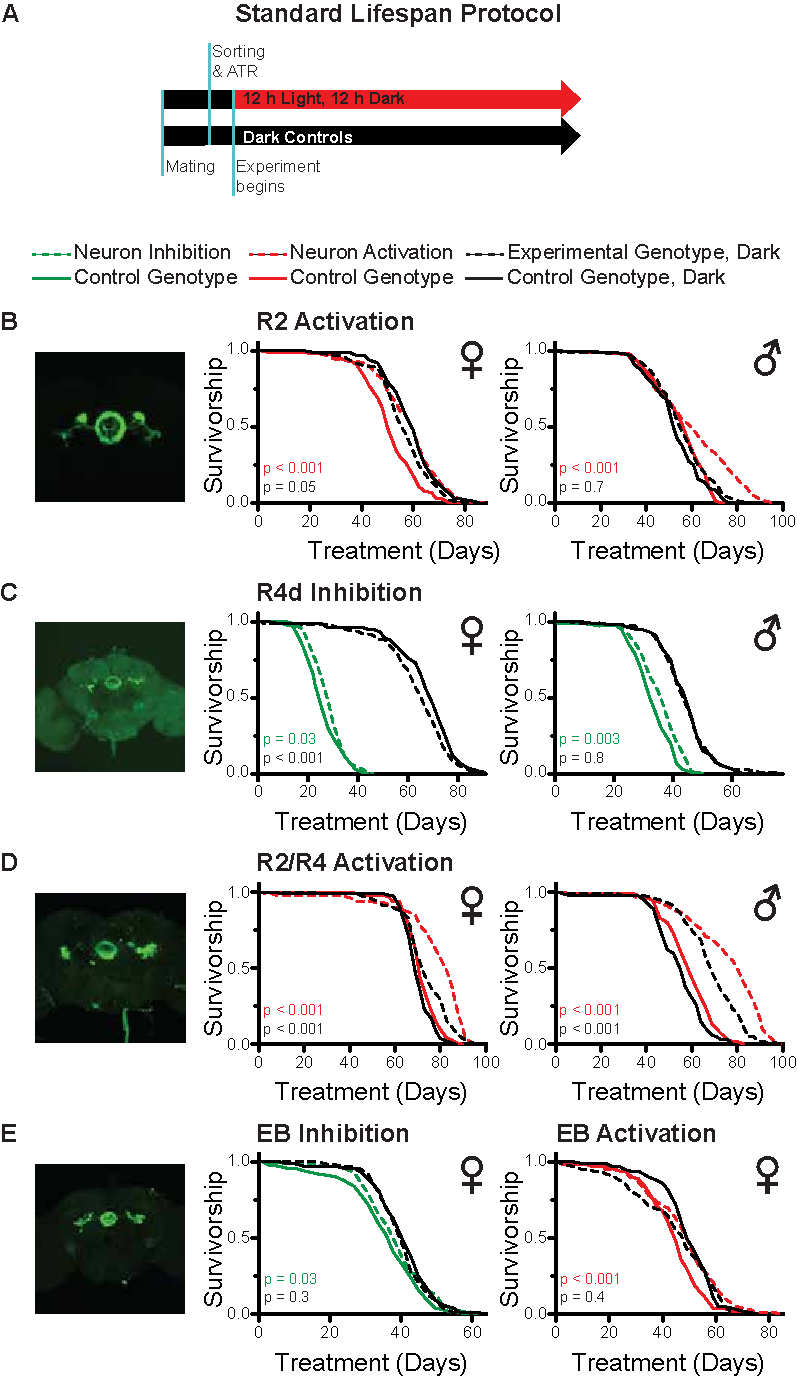
\includegraphics[width=\textwidth,height=.9\textheight,keepaspectratio]{Figs/Lifespan_Fig.pdf}
\caption{\textbf{EB manipulations extend lifespan.} Manipulation of ellipsoid body neurons R2 and R4 extends lifespan in males and females. 
(a) Flies were mated for two days, then separated by sex and sorted onto all-trans retinal food for 24 hours before optogenetic treatment began. 
(b--d) (Left) Expression patterns of drivers used in each experiment. Neurons were either activated (red lines) using UAS-CsChrimson, or inhibited (green lines) using UAS-GtACR1. Dark controls (black lines) were included for all experiments.}
\label{fig:lifespanfig}
\end{figure}

\begin{figure}[p]
\centering
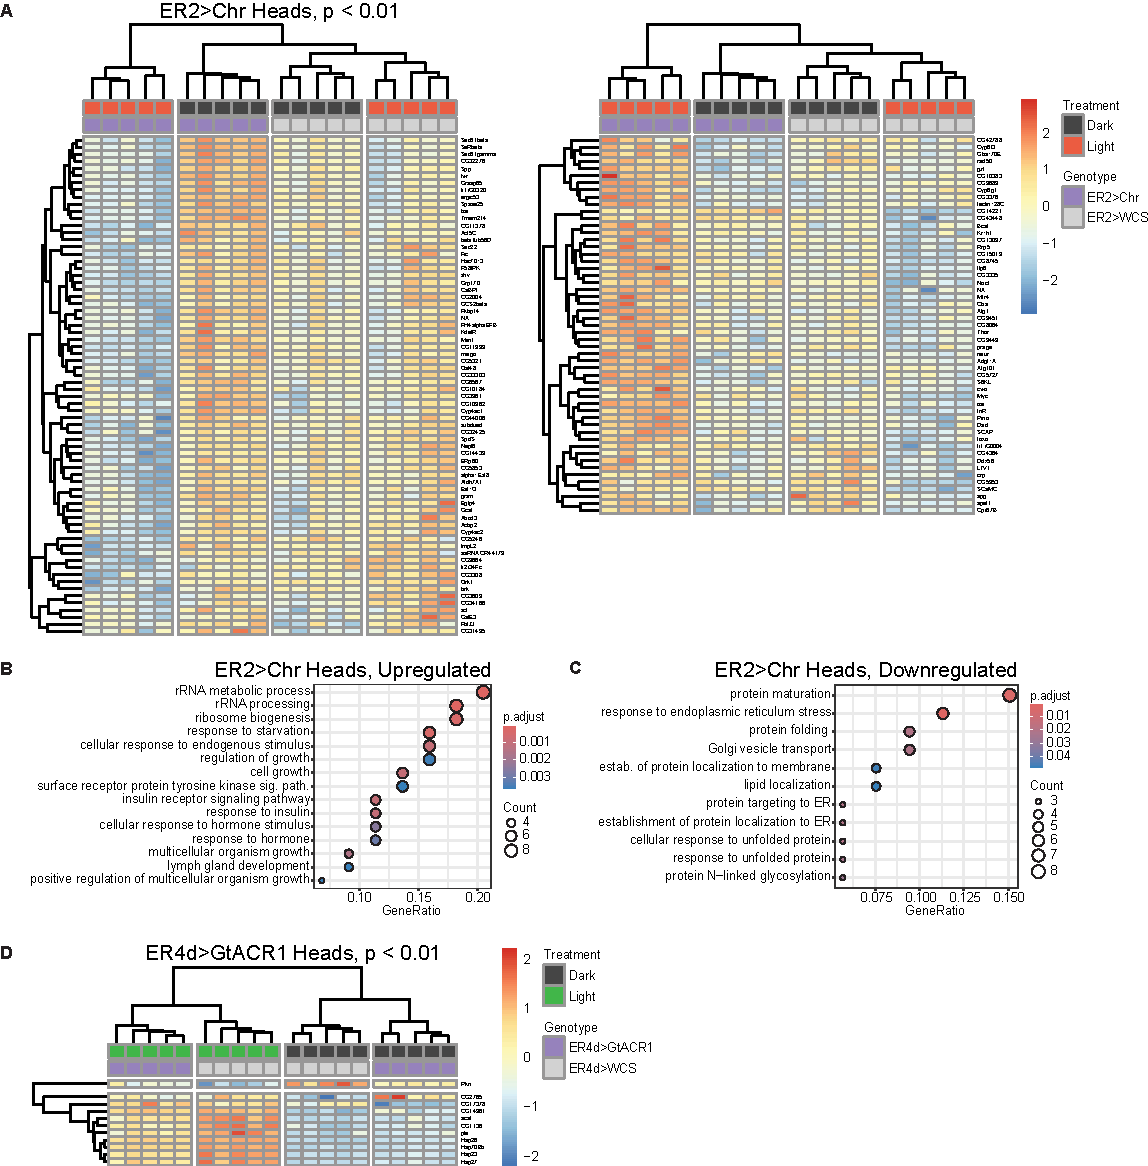
\includegraphics[width=\textwidth,height=.9\textheight,keepaspectratio]{Figs/Seq_Fig.pdf}
\caption{\textbf{EB manipulations produce distinct head transcriptomes.} Blah blah blah.}
\label{fig:seqfig}
\end{figure}

\begin{figure}[htbp]
\centering
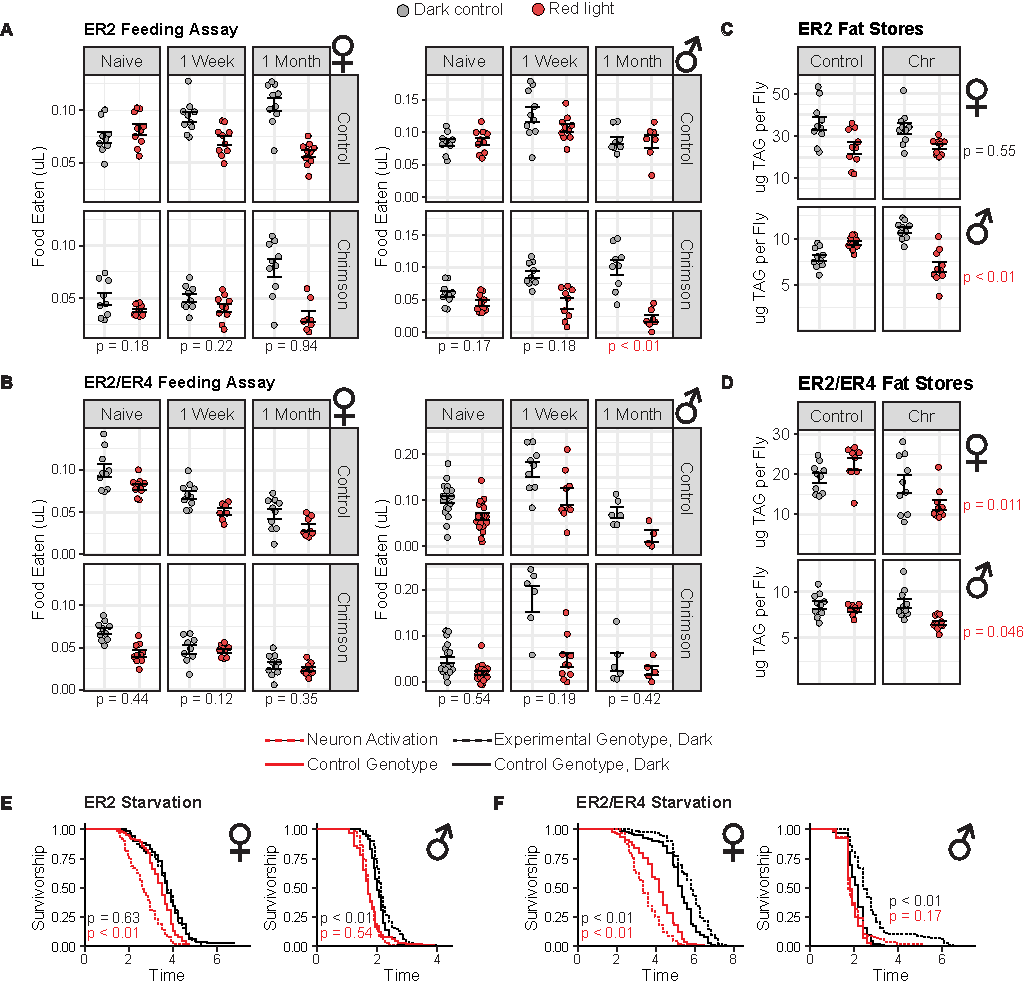
\includegraphics[width=\textwidth,height=.9\textheight,keepaspectratio]{Figs/Con-Ex_and_TAG_Fig.pdf}
\caption{\textbf{R2 and R2/R4 activation uncouples nutrient-state signaling from behavioral and physiological outputs.} \textbf{(A-D)} Interaction (Light $\times$ Genotype) p-values derived from 2-way ANOVAs. Benjamini-Hochberg correction was applied within each sex and driver, and across time points for con-ex. Female TAG points represent 5 flies; all others represent 10 flies. 
\textbf{(A)} R2-GAL4 con-ex. Female n = 8--10; male n = 7--10. 
\textbf{(B)} R2/R4-GAL4 con-ex. Female n = 7--10; male n = 18--20 (naive), 6--10 (1 week), 4--6 (1 month). 
\textbf{(C)} R2-GAL4 TAG levels. n = 10 for both sexes. 
\textbf{(D)} R2/R4-GAL4 TAG levels. Female n = 9--10; male n = 8--10. 
\textbf{(E)} R2 starvation stats. 
\textbf{(F)} R2/R4 starvation stats.}
\label{fig:conexfig}
\end{figure}

\begin{figure}[htbp]
\centering
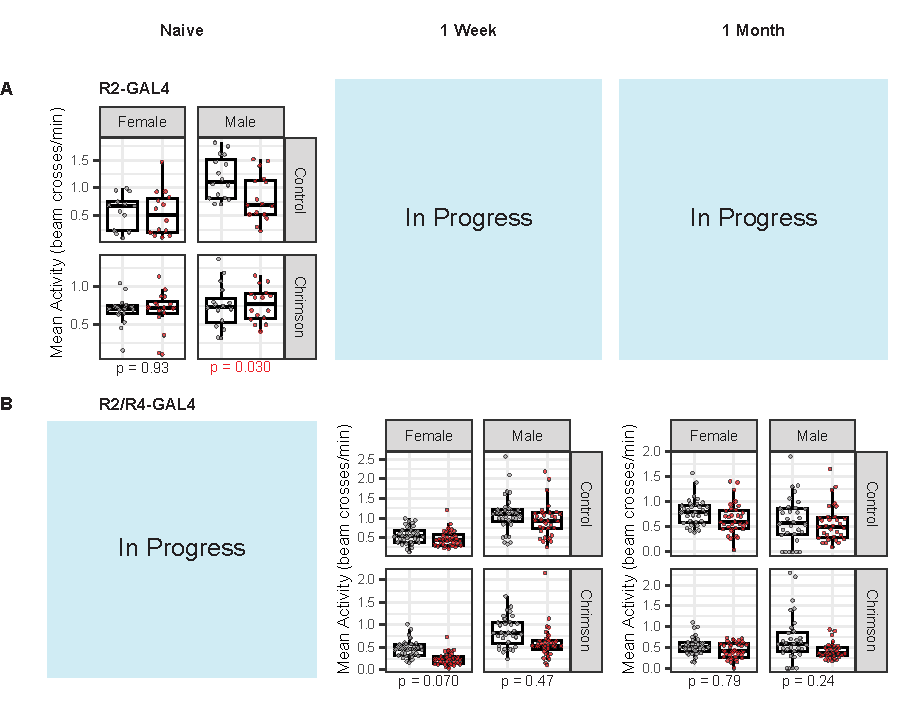
\includegraphics[scale=1]{Figs/DAMS_Fig.pdf}
\caption{\textbf{R2 and R2/R4 activaiton does not significantly affect motor activity.} R2 n = 13-16. R2/R4 n = 32. Interaction (Light $\times$ Genotype) p-values derived from 2-way ANOVAs. Benjamini-Hochberg correction was applied within each sex and driver and across time points.}
\label{fig:damsfig}
\end{figure}

\begin{figure}[htbp]
\centering
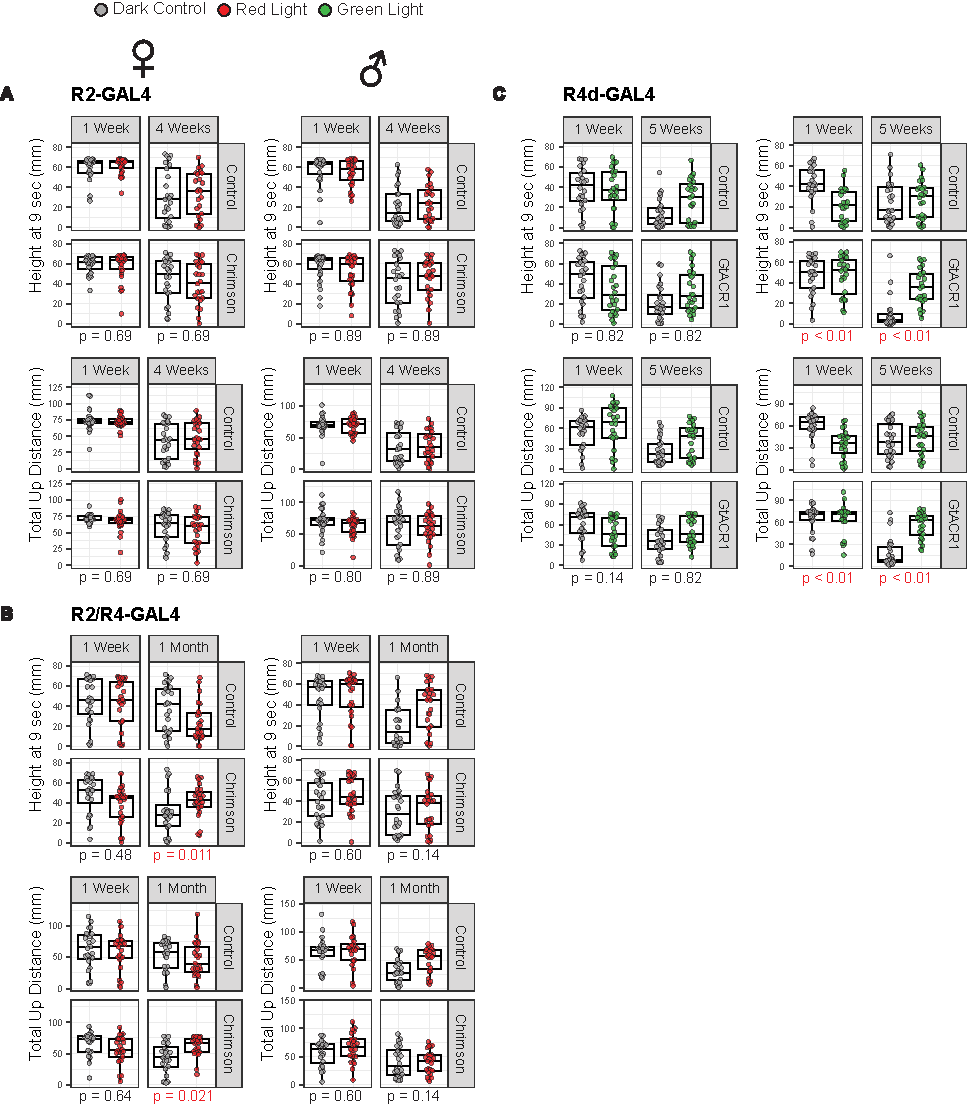
\includegraphics[scale=1]{Figs/DDrop_Fig.pdf}
\caption{\textbf{EB manipulation does not impair climbing ability.} Interaction (Light $\times$ Genotype) p-values derived from 2-way ANOVAs. Benjamini-Hochberg correction was applied within each sex and driver and across time points and climbing metrics. Points represent average of 3 trials per individual. n = 23--28.}
\label{fig:ddropfig}
\end{figure}

\begin{figure}[htbp]
\centering
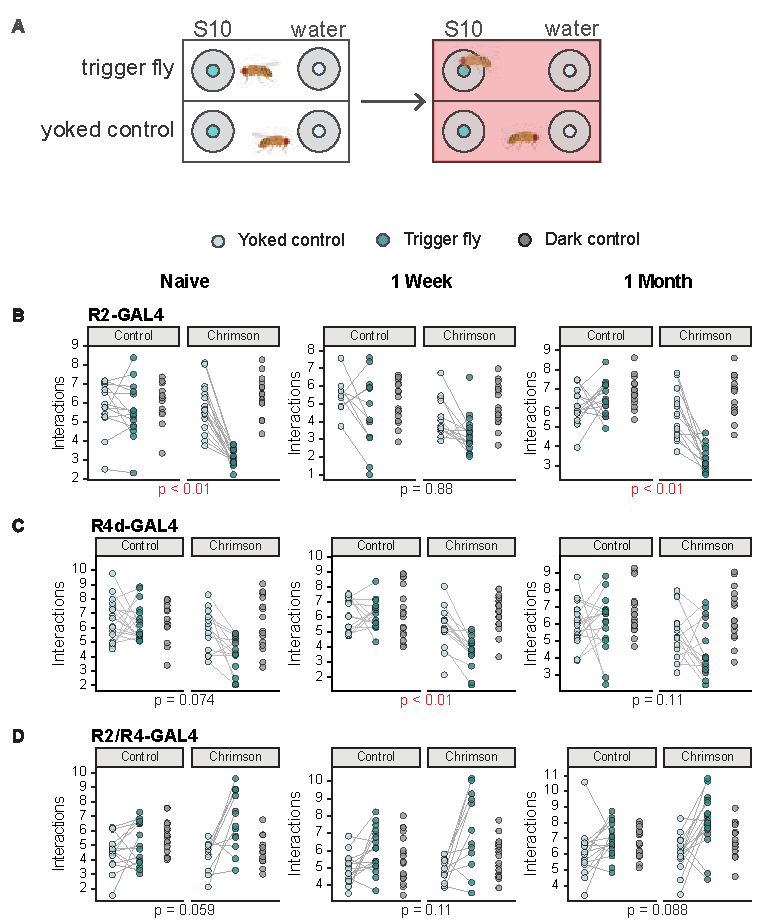
\includegraphics[scale=1]{Figs/FLIC_Fig.pdf}
\caption{\textbf{FLIC captures distinct valence states induced by EB manipulation.} Followed by desc.}
\label{fig:flicfig}
\end{figure}

\begin{figure}[p]
\centering
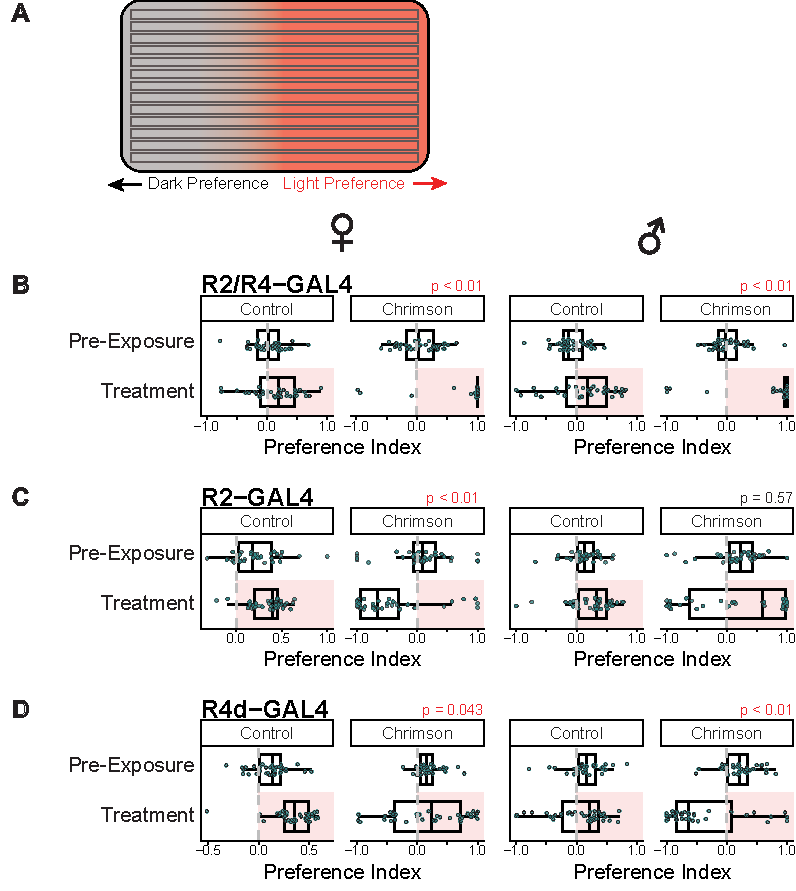
\includegraphics[width=\textwidth,height=.9\textheight,keepaspectratio]{Figs/Arena_Fig.pdf}
\caption{\textbf{Valence of EB manipulation is sex-, circuit-, and context-dependent.} Blah blah arena.}
\label{fig:arenafig}
\end{figure}